% ============================================== %
% Author: Simone Bianco
%
% Thesis Title: Efficient Parity Decision Trees and Their Connections to Logical Proofs and Total Search Problems in NP
%
% Bachelor of Science in Computer Science, Sapienza University of Rome.
%
% https://github.com/Exyss/bsc-thesis/
%
% ============================================== %

% Document Class
\documentclass[binding=0.6cm, noexaminfo, oneside]{styles/sapthesis}

% Fundamental Packages
\usepackage[dvipsnames]{xcolor}
\usepackage[english]{babel}
\usepackage[utf8]{inputenc}
\usepackage[edges]{forest}
\usepackage{microtype}
\usepackage{hyperref}
\usepackage{geometry} 
\usepackage{xspace}
\usepackage{xargs}              
\usepackage[
  backend=biber,
  style=alphabetic,
  sorting=anyt,
  minnames=3,
  minalphanames=3
]{biblatex}

% Useful Packages
\usepackage{chngcntr}
\usepackage{listings}
\usepackage{enumitem}
\usepackage[nameinlink]{cleveref}
\usepackage{caption}  
\usepackage{amssymb}
\usepackage{amsthm}
\usepackage{float}    
\usepackage[
  colorinlistoftodos,
  prependcaption,
  textsize=tiny
]{todonotes}

% Other Packages
\usepackage[Algoritmh]{algorithm}      
\usepackage{algpseudocode}

%%%% NOTE: Enable the following two lines if you want to use SapThesis' bibliography style

% \bibliographystyle{sapthesis}
% \bibliography{./references.bib}

% ================== METADATA ==================
\hypersetup{pdftitle={Master's Thesis}, pdfauthor={Simone Bianco}, colorlinks=true, urlcolor=black}
\title{Impossibility of Automated Theorem Proving for Propositional Proof Systems by Analyzing Meta-Complexity Statements}
\author{Simone Bianco}
\IDnumber{1986936}
\course{Master's Degree in Computer Science}
\courseorganizer{Faculty of Information Engineering, Computer Science and Statistics}
\AcademicYear{2025/2026}
\advisor{Prof. Nicola Galesi\\Prof. Massimo Lauria}
% \coadvisor{}
\authoremail{bianco.simone@outlook.it}
\copyyear{2026}
\thesistype{Master's Thesis}

% ================== CUSTOM ELEMENTS ==================
\usepackage{./styles/custom}

% ================== DOCUMENT ==================

\addbibresource{./references.bib}

\begin{document}

\frontmatter

\maketitle

% ================== DEDICATION ==================
\dedication{
  % \say{idk something said by someone smarter than me}\\--- not me
  something said by someone smarter than me\\--- not me
}

% ================== ABSTRACT ==================

\begin{abstract}

    % bla bla
\end{abstract}

\let\cleardoublepage\clearpage

\cleardoublepage

% ================== TABLE OF CONTENTS ==================

\hypersetup{linkcolor=black} % Print ToC in black
\setlength{\parskip}{4pt} % Vertical Spacing between elements of the ToC
\tableofcontents

\let\cleardoublepage\clearpage
\mainmatter

% ================== TYPESETTING ==================

\hypersetup{linkcolor=SapienzaRed, citecolor=SapienzaRed}          % Link colors
\counterwithout{figure}{chapter}                    % Remove chapter number from figure counter
\setlength{\parskip}{2pt}                           % Vertical spacing between paragraphs
% \setlength{\parindent}{0pt}                       % Horizontal spacing at the start of a paragraph

% ================== CHAPTERS ==================
\chapter{Introduction} \label{chap:introduction}

\section{History of the problem}

It's 1956. The genius mathematician John von Neumann is hospitalized at the Walter Reed Army Medical Hospital in Washington, USA. One year earlier, a mass was found near his collarbone, which turned out to be cancer, probably caused by exposure to radiation at the Los Alamos National Laboratory during World War II \cite{vn_biography, vn_book}. After his condition improved thanks to a successful treatment, his colleague and friend Kurt Gödel sent a letter to express solidarity for his diagnosis, hoping for a full recovery. To keep von Neumann busy during his hospital stay, Gödel proposed his friend a seminal problem of fundamental interest both for logic and computer science.

\begin{quote}
    \say{One can obviously easily construct a Turing machine, which for every formula $F$ in first order predicate logic and every natural number $n$, allows one to decide if there is a proof of $F$ of length $n$ (length = number of symbols). Let $\psi(F,n)$ be the number of steps the machine requires for this and let $\varphi(n) = \max_F \psi(F,n)$. The question is how fast $\varphi$(n) grows for an optimal machine. One can show that $\varphi(n) \ge kn$.
    \newline
    If there really were a machine with $\varphi(n) \sim kn$ (or even $\sim kn^2$), this would have consequences of the greatest importance. Namely, it would obviously mean that in spite of the undecidability of the Entscheidungsproblem, the mental work of a mathematician concerning Yes-or-No questions could be completely replaced by a machine. After all, one would simply have to choose the natural number $n$ so large that when the machine does not deliver a result, it makes no sense to think more about the problem.}

    \hfill Gödel to von Neumann, Princeton, 20 March 1956 \cite{godel_letter, sipser_pnp}
\end{quote}

In a less formal way, Gödel's question asks if there is an efficient algorithm capable of deciding if a given mathematical statement has a proof of some given length. In modern times, the above problem became known as the \textit{Proof Size Problem} (PSP) \cite{psp_res, psp_res_2, pap}. Sadly, no reply from Von Neumann is known. During his long hospital stay, von Neumann's mental health rapidly declined due to his extreme thanatophobia, the fear of impending death \cite{vn_biography}. Almost a year later after being hospitalized, von Neumann died \cite{vn_book, vn_biography}.

When restricted from first-order predicate logic to propositional logic, Gödel's question becomes an historic precursor of the \textit{$\mathsf{P}$ vs.\,$\mathsf{NP}$} question, which asks whether problems whose solutions are easy to double-check, i.e. problems that lie in the class $\mathsf{NP}$, are also easy to solve from scratch, i.e. if they also lie in the class $\mathsf{P}$ \cite{cook_sat, levin_fsat}. The most interesting problems in $\mathsf{NP}$ are the so-called $\mathsf{NP}$-complete problems, that being problems in $\mathsf{NP}$ whose efficient solution would imply an efficient solution for all $\mathsf{NP}$ problems, i.e. $\mathsf{P} = \mathsf{NP}$. The current state of the art conjectures that $\mathsf{P} \neq \mathsf{NP}$, meaning that these so-called complete problems cannot be efficiently solved in their general case (see \Cref{sec:complexity} for more detailed information).

If this were the case, no algorithm could be substantially better than something based on a \textit{brute force} approach, the idea of testing every candidate solution in the search space defined by the problem itself. For instance, if a problem asks to determine if there is a sub-structure with a specific property, the brute force approach tests every possible sub-structure. In his letter, Gödel himself states that he sees no better approach than that of reducing the search space through clever techniques. Over the years, researchers began to explore the problem for \textit{propositional proof systems} \cite{cook_proof_compx, kraj_book, galesi_toran}, i.e. logical systems that use restricted rules to find proofs of propositional statements, confirming Gödel's hypothesis \cite{psp_res, psp_res_2}.

Although $\mathsf{P} \neq \mathsf{NP}$ would rule out efficient proof-search algorithms, the practical demand for Automated Theorem Proving (ATP) \cite{handbook_sat} kept growing as society advanced. This branch of computer science is applied in all areas where absolute reliability is required (hardware design, software verification, modern mathematics, \dots). To address this issue, computer scientists and logicians started investigating a closely related problem, referred to as automatability \cite{fis_int_weak_aut,res_wphard}. \textit{Automatability} asks if for a fixed proof system one can find an algorithm that returns a proof of a given statement with an at most polynomial blow-up with respect to the size of the shortest proof.

A central discovery of modern proof complexity is that natural propositional proof systems are not automatable under some widely believed complexity assumption, such as standard cryptographic assumptions \cite{kraj_pud_crypto, fis_int_weak_aut,ac0_crypto} or even $\mathsf{P} \neq \mathsf{NP}$ \cite{res_nphard,alg_nphard,cp_nphard,resk_nphard,ac0f_nphard}. Previously, similar results were known under stronger hypotheses \cite{res_wphard, res_hard_proofs,pc_wphard}. These results highlight a certain paradox in the world of proof search. One would expect that a more expressive proof system would be capable of achieving remarkably short proofs, making it easier to generate proofs. However, the very same increase in expressive power implies that the search space of those proofs may be so unstructured that no algorithm can find them faster than brute force. In other words, it seems that if an algorithm fails to discover a short proof that is guaranteed to exist then the fault lies not in the algorithm, but in the proof space itself.

These findings culminate into the brand new concept of analyzability \cite{pap}. While automatability evaluates whether an algorithm can efficiently output a proof bounded by the size of the shortest existing proof in a fixed system, \textit{analyzability} inspects the structural complexity of its search space. In particular, we are interested in understanding if proofs of lower bounds can leak information about the formula. For instance, we may be able to learn some information about the satisfiability of a formula by investigating what allows a proof system to achieve short proofs of the formula's lower bounds.

\section{Thesis structure and contributions (TODO)}

\cleardoublepage
\chapter{Preliminaries} \label{chap:preliminaries}

\section{Propositional logic}

Propositional logic serves as the foundational mathematical framework for reasoning over declarative statements using Boolean truth values and formal logical operators. For our purposes, we will be interested in a fragment of propositional logic that works with finite amount of elements. For a more in depth explanation of propositional logic covering topics necessary to understand this work, the reader is referred to \cite{logic_book,kraj_book,galesi_toran}.

Let $\mathrm{Var} = \{x_1, \ldots, x_n\}$ denote a non-empty, finite set of atomic propositional symbols, called \textit{variables}, and let $\mathscr{O} = \{\land, \lor, \lnot, \to, \leftrightarrow\}$ be the set of Boolean logical connectives. Each of these connectives represents, respectively, the concept of conjunction, disjunction, negation, implication and logical equivalence. By recursively combining these connectives, starting from variables, we can build formulas that fully express sentences and properties. For instance, the sentence \curlyquotes{I'll take my umbrella and my boots if it rains} can be modeled by the formula $R \to (U \land B)$.

\begin{definition}
  The set of formulas $\mathrm{Fml}$ is defined as the free algebra generated by $\mathrm{Var}$ and $\mathscr{O}$. That is, $\mathrm{Fml}$ is the smallest set satisfying the following three conditions:
  \begin{itemize}
    \item $\mathrm{Var} \subset \mathrm{Fml}$;
    \item If $\varphi \in \mathrm{Fml}$ then $\neg \varphi \in \mathrm{Fml}$;
    \item If $\varphi, \psi \in \mathrm{Fml}$ and $\circ \in \mathscr{O}\setminus \{\lnot\}$ then $(\varphi \circ \psi) \in \mathrm{Fml}$.
  \end{itemize}
\end{definition}

The set $\mathrm{Fml}$ defines propositional logic from a syntactical point of view, i.e. how correct formulas are written. To give meaning to the formulas, we have to also define it from a semantic perspective using \textit{assignments}.

\begin{definition}
  An assignment is a mapping $\alpha : \mathrm{Var} \to \{0,1\}$ that sets a truth value to each variable.
\end{definition}

By extension, each assignment $\alpha$ over variables induces an assignment $\widehat{\alpha} : \mathrm{Fml} \to \{0,1\}$ through the semantical meaning of the logical connectives:
  \begin{itemize}
    \item $\widehat{\alpha}(\lnot \varphi) = 1$ if and only if $\widehat{\alpha}(\varphi) = 0$
    \item $\widehat{\alpha}(\varphi \land \psi) = 1$ if and only if $\widehat{\alpha}(\varphi) = \widehat{\alpha}(\psi) = 1$
    \item $\widehat{\alpha}(\varphi \lor \psi) = 0$ if and only if $\widehat{\alpha}(\varphi) = \widehat{\alpha}(\psi) = 0$
    \item $\widehat{\alpha}(\varphi \to \psi) = 1$ if and only if $\widehat{\alpha}(\psi) = 1$ whenever $\widehat{\alpha}(\varphi) = 1$ holds
    \item $\widehat{\alpha}(\varphi \leftrightarrow \psi) = 1$ if and only if $\widehat{\alpha}(\varphi \to \psi) = \widehat{\alpha}(\psi \to \varphi) = 1$
  \end{itemize}

\begin{table}
  \centering
  \begin{tabular}{cc|ccccc}
    \toprule
    $ \varphi $ & $ \psi $ & $ \neg \varphi $ & $ \varphi \land \psi $ & $ \varphi \lor \psi $ & $ \varphi \rightarrow \psi $ & $ \varphi \leftrightarrow \psi $ \\
    \midrule
    1 & 1 & 0 & 1 & 1 & 1 & 1 \\
    1 & 0 & 0 & 0 & 1 & 0 & 0 \\
    0 & 1 & 1 & 0 & 1 & 1 & 0 \\
    0 & 0 & 1 & 0 & 0 & 1 & 1 \\
    \bottomrule\\
  \end{tabular}
  \caption{Summary of truth assignments for logical connectives in $\mathscr{O}$.}
  \label{tab:propositional_truth_table}
\end{table}

We will abuse notation throughout this whole work by using $\alpha$ instead of $\widehat{\alpha}$. Assignments can be partial or total. A \textit{partial assignment} is an assignment defined only on a subset of variables, i.e. it is a partial function. Variables $x_i$ for which the assignment is not defined can be viewed as if they were mapped to a special symbol, $\alpha(x_i) = *$. A \textit{total assignment}, instead, assigns a value to all variables of $\mathrm{Var}$.

Next, we list a series of standard definitions that will be extensively utilized in the next chapters. A formula $\varphi \in \mathrm{Fml}$ is said to be \textit{satisfiable} if there is at least one assignment $\alpha$ such that $\alpha(\varphi) = 1$. When all possible assignments satisfy a formula, we refer to that formula as a \textit{tautology} (or valid formula). Clearly, $\varphi$ is a tautology if and only if $\lnot \varphi$ is unsatisfiable.

Two formulas $\varphi$ and $\psi$ are said to be \textit{logically equivalent}, written $\varphi \equiv \psi$, when for each assignment $\alpha$ it holds that $\alpha(\varphi) = \alpha(\psi)$. Logical equivalences often allow us to rewrite formulas in a way that is more convenient for the current context. For instance, \textit{De Morgan's rule} states that $\lnot(\varphi \land \psi) \equiv \lnot \varphi \lor \lnot \psi$ and, similarly, that $\lnot(\varphi \lor \psi) \equiv \lnot \varphi \land \lnot \psi$.

Given a Boolean variable $x$, a \textit{literal} $\ell$ of $x$ is either the variable $x$ itself or its negation $\lnot x$. A \textit{clause} is a disjunction of literals, $C = \ell_1 \lor \ldots \lor \ell_k$, while a \textit{term} is a conjunction of them, $T = \ell_1 \land \ldots \land \ell_t$. A \textit{conjunctive normal form} (CNF) formula $\varphi$ is a conjunction of $m$ clauses $C_1, \ldots, C_m$. Similarly, a \textit{disjunctive normal form} (DNF) formula is a disjunction of $s$ terms $T_1, \ldots, T_s$. Any formula can be written as a logically equivalent CNF or a logically equivalent DNF. For instance, the formula $\varphi = ((x_1 \lor \lnot x_2) \land x_3) \lor x_4$ can be converted into the CNF and DNF formulas written below:
\begin{equation}
  \label{eq_1}
  (x_1 \lor \lnot x_2 \lor x_4) \land (x_3 \lor x_4)
\end{equation}
\begin{equation}
  \label{eq_2}
  (x_1 \land x_3) \lor (\lnot x_2 \land x_3) \lor x_4
\end{equation}

A \textit{restriction} of a CNF formula $\varphi \in \mathrm{Fml}$ over an assignment $\alpha$ is a formula $\varphi_{\upharpoonright_{\alpha}}$ obtained from $\varphi$ through the following procedure. For each literal $\ell$ with $\alpha(\ell) = b$, where $b \in \{0,1\}$, we modify $\varphi$ in the following way:
\begin{itemize}[nosep]
  \item If $b = 0$, we remove the literal $\ell$ from each clause of $\varphi$;
  \item If $b = 1$, we remove each clause of $\varphi$ that contains $\ell$.
\end{itemize}

For instance, consider again the CNF formula in \Cref{eq_1}. When restricted under the assignment $\alpha = \{x_2 \mapsto 1, x_3 \mapsto 1\}$, the formula becomes $x_1 \lor x_4$.

\section{Encodings of combinatorial principles}

Instead of working with CNF formulas that do not follow a structure, throughout this work we will focus on CNF formulas that encode combinatorial principles \cite{kraj_book,handbook_sat,galesi_toran}. Intuitively, these formulas make proving computational results easier thanks to their underlying principles \cite{kraj_book,galesi_toran}. For instance, the CNF formula $\mathrm{PHP}^{m}_n$ describing the \textit{Pigeonhole Principle} --- the combinatorial principle stating that $m$ pigeons cannot be mapped to $n$ holes when $m > n$ --- allows us to imagine a partial assignment for this formula as a partial mapping between pigeons and holes.

To encode combinatorial principles we usually rely on mathematical relations. Let $X$ be a finite set. For each pair $i,j \in X$ we define a \textit{Boolean indicator variable} $x_{i,j}$. Through these variables, any total assignment on the variables $\{x_{i,j}\}_{i,j \in X}$ corresponds to a relation $R_{\alpha} \subseteq X \times X$ with the intended meaning of $\alpha(x_{i,j}) = 1$ if and only if $R(i,j)$ holds. Any formula satisfied by an assignment describes a property satisfied by the relation described by such assignment.

As an example, consider the formula $x_{i,j} \land x_{j,k}$. This formula may be interpreted as the statement \curlyquotes{$j$ stands between $i$ and $k$} under some order relation $\preceq$. Another possible interpretation is the statement \curlyquotes{there are two edges $(i,j)$ and $(j,k)$} under some edge relation describing a graph.

As long as $X$ is finite, it is always possible to define a finite set of variables that express the relation $R$ over $X$ in propositional form. More complex properties of relations are described through the \textit{existential} and \textit{universal quantifiers}, $\exists$ and $\forall$. Indeed, such statements can also be encoded as propositional formulas --- again, assuming $X$ is finite --- by translating them, respectively, into a chain of logical ORs or logical ANDs, $\lor$ and $\land$. For instance, the statement \curlyquotes{there is an element $i$ in $X$ such that for all elements $j$ in $X$ it holds that $R(i,j)$} can be expressed as the Boolean disjunction ranging over all the elements $i$ of $X$ with a nested Boolean conjunction of $x_{i,j}$, ranging over all elements $j$ of $X$:
\begin{equation}
  \bigvee_{i \in X} \bigwedge_{j \in X} x_{i,j}
\end{equation}

Going back to combinatorial principles, consider again the Pigeonhole Principle. This simple counting principle captures one of the most basic primitives of mathematics. Since the pigeonhole principle entails a counting argument, it has been considered as a prominent example of formula that is hard to prove for reasoning systems that have no rules that allow them to count \cite{php_lower, php_lower_2,php_easy,kraj_book,galesi_toran}.

Formally, the principle says that if $f$ is a total mapping from $[m] = \{1, \ldots, m\}$ to $[n] = \{1, \ldots, n\}$ with $m > n$ then $f$ has a \textit{collision}, that is, there are two pigeons $i,i' \in [m]$ with $i \neq i'$ mapped to the same hole, meaning $f(i) = j$ and $f(i') = j$. In first-order logic, this can be expressed as:
\begin{equation}
  (\forall i \in [m] \, \exists j \in [n] \, f(i) = j) \to \exists i,i' \in [m] \, \exists j \in [n] \, i \neq i' \land f(i) = j \land f(i') = j
\end{equation}

By introducing the Boolean variables $p_{i,j}$ with the intended meaning of $\alpha(p_{i,j}) = 1$ if and only if pigeon $i$ goes to hole $j$, i.e. $f(i) = j$, the above formula can be translated into a propositional formula as follows:
\begin{equation}
  \rbk{\bigwedge_{i \in [m]} \bigvee_{j \in [n]} p_{i,j}} \to \bigvee_{\substack{i,i' \in [m] :\\ i \neq i'}} \bigvee_{j \in [n]} p_{i,j} \land p_{i',j}
\end{equation}

Since the underlying combinatorial principle is always true, we know that the formula must be a tautology. For many applications, its negated formula is often needed. Using the logical equivalence $\varphi \to \psi  \equiv \lnot \varphi \lor \psi$, this negated formula can be described by the Boolean conjunction of the following $m + n\binom{m}{2}$ clauses:
\[\begin{array}{clr}
  p_{i,1} \lor \ldots \lor p_{i,n} & \forall i \in [m] & (\text{Pigeon axioms})\\
  \lnot p_{i,j} \lor \lnot p_{i', j} & \forall i,i' \in [m] \text{ with $i \neq i'$ and } \forall j \in [n] & (\text{Hole axioms})\\
\end{array}\]

This last propositional formula is referred to as $\mathrm{PHP}^{m}_n$. Proving that $\mathrm{PHP}^{m}_n$ is unsatisfiable is equivalent to proving that $\lnot \mathrm{PHP}^{m}_n$ is a tautology. Many variants of this unsatisfiable formula are used in many applications, adding or removing some properties, such as functionality, surjectivity and bijectivity \cite{php_variants}. In \Cref{sec:rPHP} we will work with one such variant.


\begin{figure}[t]
  \centering
    \resizebox{0.6\textwidth}{!}{
        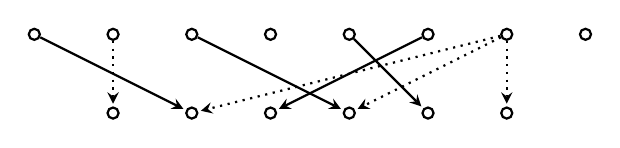
\begin{tikzpicture}[->,>=stealth,shorten >=1pt,auto,node distance=1cm, thick,main node/.style={scale=0.9,circle,draw,font=\sffamily\normalsize},
        block/.style={rectangle, draw, minimum width = 60, minimum height = 20, rounded corners = 6pt}, small circle/.style={circle, draw, inner sep=0pt, minimum size=4pt}]

            % Pigeons

            \foreach \b [
                evaluate = \b as \bprev using {int(\b-1)},
            ] in {0,1,2,3,4,5,6,7} {
                \ifnum\b=0
                  \node [small circle] (p\b) [] {};
                \else
                  \node [small circle] (p\b) [right of = p\bprev] {};
                \fi
            }

            % Holes

            \foreach \b [
                evaluate = \b as \bprev using {int(\b-1)},
            ] in {0,1,2,3,4,5} {
                \ifnum\b=0
                  \node [small circle] (h\b) [below of = p1] {};
                \else
                  \node [small circle] (h\b) [right of = h\bprev] {};
                \fi
            }

            % Pigeons

            \path[every node/.style={font=\sffamily\small}]
                  (p0) edge (h1)
                  (p1) edge[dotted] (h0)
                  (p2) edge (h3)
                  (p4) edge (h4)
                  (p5) edge (h2)
                  (p6) edge[dotted] (h1)
                  (p6) edge[dotted] (h3)
                  (p6) edge[dotted] (h5)
                ;
        \end{tikzpicture}
    }
    \caption{Graphical representation of a partial assignment on $\mathrm{PHP}^8_6$. Each edge is a variable $p_{i,j}$. Solid edges are assigned as true, missing edges are assigned as false and dotted edges are unassigned.}
    \label{fig:php}
\end{figure}

\section{Computability}

Depending on the objective, a problem can ask for a binary answer, a specific solution structure or the best possible solution out of many. We divide these problems into three categories: \textit{decision}, \textit{search} and \textit{optimization} \cite{sip_book,papad_book}. A decision problem is a problem for which we are asked to determine if a chosen property holds for a given a instance of the problem. A search problem, instead, asks to find some structure that certifies the validity of the chosen property. Similarly, an optimization problem asks us to find the optimal structure among all the available ones. It is easy to see that these three ideas form some sort of hierarchy between types of problems. In general, optimization problems are at least as hard as search problems, which in turn is at least as hard as decision problems. For $\mathsf{NP}$-complete problems (see \Cref{sec:complexity}), search and decision are generally polynomially equivalent. This property is known as \textit{self-reducibility} \cite{decision_vs_search,papad_book}.

We face these types of problems every day in our life. For instance, suppose that we want to reach a destination $B$ from a starting point $A$. If we are interested in finding the \textit{shortest} route between point $A$ and $B$, this becomes an optimization problem. If we want to find a route between the two sites, without caring about its length, this becomes a search problem. If, instead, we want to just establish the existence of at least one route, this becomes a decision problem.  

Let $\Sigma$ be a finite set of symbols (e.g. $\Sigma = \{a,b,c, 0, \$, 3, x, \ldots\}$), referred to as \textit{alphabet}, and let $\Sigma^*$ be the infinite set of all finite strings formed by characters taken from that alphabet. Any subset $L \subseteq \Sigma^*$ is referred to as a \textit{language}. Typically, we are interested in the case where $\Sigma = \{0,1\}$.

Consider a binary predicate $P : \Sigma^* \to \{0,1\}$ representing some property, meaning that $P(x) = 1$ means that the property holds for the input instance $x$ and $P(x) = 0$ means that it does not. Let $R_P \subseteq \Sigma^* \times \Sigma^*$ be the binary relation such that $R_P(x,y)$ holds if and only if $y$ certifies the fact that $P(x) = 1$. We refer to $\mathrm{Sol}_P(x) = \{y \in \Sigma^* \mid R_P(x,y)\}$ as the set of \textit{solutions} (or \textit{witnesses}) for the instance $x$ over the property $P$.

\begin{definition}
  The decision problem of $P$ is defined as the language $\Pi_{\text{dec}}^P = \{x \in \Sigma^* \mid \mathrm{Sol}_P(x) \neq \varnothing\}$. The problem $\Pi_{\text{dec}}^P$ is said to be decidable (or computable) if there is an algorithm $\mathcal{A}$ such that $\mathcal{A}(x) = 1$ when $\mathrm{Sol}_P(x) \neq \varnothing$ and $\mathcal{A}(x) = 0$ otherwise.
\end{definition}

We observe that the above definition of computability for decision problem can also be stated as the existence of an always-halting algorithm $L(\mathcal{A}) =\Pi_{\text{dec}}^P$. Moreover, we also observe that the above definition could've been stated without the use of the binary relation $R_P$ since $\Pi_{\text{dec}}^P = \{x \in \Sigma^* \mid P(x) = 1\}$ is an equivalent definition. In this setting, the definition is given using $R_P$ only for consistency with search and optimization problems. In fact, for the other two types of problems binary relations are necessary due to the fact that one instance may have more than one possible witness. For instance, there may be more than one (optimal) route from point $A$ to point $B$.

\begin{definition}
  The search problem of $P$ is defined as the binary relation $\Pi_{\text{search}}^P = R_P$. The problem $\Pi_{\text{search}}^P$ is said to be solvable (or computable) if there is an algorithm $\mathcal{A}$ such that $\mathcal{A}(x) \in \mathrm{Sol}_P(x)$ when $\mathrm{Sol}_P(x) \neq \varnothing$ and $\mathcal{A}(x) = \bot$ otherwise.
\end{definition}

Here, the symbol $\bot$ is used to represent the fact that no solution exists for the given input instance. The definition allows any algorithm computing the problem to return a different solution on each execution. Optimization problems require an additional component: a \textit{cost function} $c : \Sigma^* \times \Sigma^* \to \R$ expressing the optimality of the solution for the given instance. We denote the set of optimal solutions as $\mathrm{Opt}_P(x) = \{y \in \mathrm{Sol}_P(x) \mid c(x,y) = \max_{z \in \mathrm{Sol}_P(x)} c(x,z)\}$. Notice that each maximization problem can be rewritten as an equivalent minimization problem. 

\begin{definition}
  The optimization problem of $P$ over $c$ is defined as the binary relation $\Pi_{\text{opt}}^P = \{(x,y) \in \Sigma^* \times \Sigma^* \mid y \in \mathrm{Opt}_P(x)\}$. The problem $\Pi_{\text{opt}}^P$ is said to be solvable (or computable) if there is an algorithm $\mathcal{A}$ such that $\mathcal{A}(x) \in \mathrm{Opt}_P(x)$ when $\mathrm{Sol}_P(x) \neq \varnothing$ and $\mathcal{A}(x) = \bot$ otherwise.
\end{definition}

As previously stated, these three categories form a hierarchy of problems. This is clear from their own definitions: any algorithm computing an optimization problem also computes a search problem and any algorithm computing a search problem can be adapted into one that computes a decision problem.

\section{Computational complexity}
\label{sec:complexity}
In his seminal work, Turing \cite{turing} proved that some problems are \textit{undecidable}, meaning that there is no algorithm that can compute them exactly. Following his work, the pioneers of computer science started noticing that even though many problems can be computed, the algorithms computing them would take too many resources, making them infeasible to process for large inputs. In particular, they focused on two main measures: \textit{time} and \textit{space} \cite{complexity_measures,sip_book,arora_barak}. 

\begin{definition}
  Let $\mathcal{A}$ be an algorithm and let $t, s \colon \N \to \R^+$ be two functions. We say that $\mathcal{A}$ \emph{runs in time} $t$ if on every input $x$ the algorithm halts after at most $t(|x|)$ steps and that $\mathcal{A}$ \emph{runs in space}
  $s$ if on every input $x$ it uses at most $s(|x|)$ memory cells.
\end{definition}

These two complexity measures are intrinsically related one to another and they are, usually, negatively correlated. Generally, if we allow our algorithm to use more space then the computation can be sped up by saving partial computations, while if we want to lower the amount of space needed then these partial computations have to be calculated each time they are required. Larger inputs require larger amounts of computational resources, making the values $t(n)$ and $s(n)$ proportional to the size $n$ of the input.

Usually, we work with these measures as the input length grows asymptotically. In particular, borrowing notation from standard calculus, we are interested in bounding costs from above and below, up to some constant factor. Let $f,g : \N \to \R^+$ be two functions. We say that:
  \begin{itemize}[nosep]
    \item $f(x)$ is in $O(g(x))$ when there are two constants $c,n_0 > 0$ such that $\forall n \geq n_0$ we have $f(n) \leq c \cdot g(n)$;
    \item $f(x)$ is in $\Omega(g(x))$ when there are two constants $c,n_0 > 0$ such that $\forall n \geq n_0$ we have $f(n) \geq c \cdot g(n)$;
    \item $f(x)$ is in $\Theta(g(x))$ when $f(x)$ is both in $O(g(x))$ and $\Omega(g(x))$;
    \item $f(x)$ is in $o(g(x))$ when for each constant $c > 0$ there is a constant $n_0 > 0$ such that $\forall n \geq n_0$ we have $f(n) < c \cdot g(n)$.
  \end{itemize}

The main goal of computational complexity is establishing what can and cannot be solved under some complexity measure constraints. In real world situations, any algorithm with runtime larger than $O(n^3)$ is considered impractical since it requires too much time for large inputs. Nonetheless, complexity theorists use this to their advantage: if a problem cannot be solved even when allowing this constraint to be any form of \textit{polynomial time}, i.e. time $O(n^c)$ for some $c > 0$, the problem is ruled out as \textit{intractable}. Therefore, in this context efficient and polynomial-time are considered synonyms of each other. The class of all efficiently solvable decision problems is denoted with $\mathsf{P}$ and the same holds for $\mathsf{FP}$, the class of efficiently solvable search problems \cite{cobham_p,arora_barak}.

\begin{definition}
  We define $\mathsf{P}$ as the class of decision problems solvable in polynomial time by an algorithm, i.e. in time $O(n^c)$ for some $c > 0$. Similarly, $\mathsf{FP}$ is the class of search problems solvable in polynomial time.
\end{definition}

The aforementioned $\mathsf{P}$ vs. $\mathsf{NP}$ question (or $\mathsf{FP}$ vs. $\mathsf{FNP}$ for search problems) asks to settle if the class of efficiently solvable problems corresponds to the class of efficiently verifiable problems. Here, a \textit{verifier} for a problem $L$ is an algorithm that takes an additional input $w$, referred to as the \textit{witness}, and uses it to check if $x \in L$ holds or not. Usually, this witness is a string that describes a real solution of the problem for the given input. The length of the witness must be bounded by at most a polynomial with respect to the input length.

\begin{definition}
  We define $\mathsf{NP}$ as the class of decision problems verifiable in polynomial time by a verifier. In particular, for an $\mathsf{NP}$ language with verifier $V$, it holds that $x \in L$ if and only if $\exists w \in \Sigma^*$ for which $V(x,w) = 1$ and $\abs{w} \leq O(\abs{x}^c)$ for some $c > 0$.
\end{definition}

By definition, we have that $\mathsf{P} \subseteq \mathsf{NP}$ since if a problem is efficiently solvable then we can just ignore the given witness and solve the problem. Hence, the $\mathsf{P}$ vs. $\mathsf{NP}$ question asks to settle if this inclusion also holds in the converse direction, i.e.  $\mathsf{NP} \subseteq \mathsf{P}$. After more than 50 years of scientific literature studying this problem and its ramifications, researchers conjecture that the answer to this problem is negative \cite{sipser_pnp,arora_barak, aaronson_survey}.

\begin{conjecture}
  $\mathsf{P} \neq \mathsf{NP}$
\end{conjecture}

For our purposes, we will assume this conjecture to be true. Another class of our interest is the class $\mathsf{coNP}$, defined as the set of all problems whose complement is verifiable in polynomial time.

\begin{definition}
  $\mathsf{coNP} = \{L \subseteq \Sigma^* \mid \overline{L} \in \mathsf{NP}\}$.
\end{definition}

it is easy to see that problems that lie in $\mathsf{coNP}$ admit a verifier that uses witnesses to discard invalid input instances: if $w$ is a witness for the membership of $x$ in $\overline{L}$ then $w$ is also a witness for the non-membership of $x$ in $L$. In other words, a problem is in $\mathsf{NP}$ if its correct instances can be efficiently verified, while a problem is in $\mathsf{coNP}$ if the same holds for incorrect instances. 

Again, it is easy to see that $\mathsf{P} \subseteq \mathsf{coNP}$, but the converse is not known and it is actually a question equivalent to establishing that $\mathsf{P} = \mathsf{NP}$. This is due to the fact that if a problem is efficiently solvable then its complement is also efficiently solvable (we can just negate the output of the same algorithm). This same reasoning implies that if $\mathsf{P} = \mathsf{NP}$ then $\mathsf{NP} = \mathsf{coNP}$. Therefore, proving that $\mathsf{NP} \neq \mathsf{coNP}$ could be a way of establishing that $\mathsf{P} \neq \mathsf{NP}$. It is also conjectured that $\mathsf{NP} \neq \mathsf{coNP}$: there are evident asymmetries between the hardness of witnessing that something holds and that of witnessing something does not hold both in mathematics and computer science \cite{cook_proof_compx}.

\begin{conjecture}
  $\mathsf{NP} \neq \mathsf{coNP}$
\end{conjecture}

Going upwards with time complexity, we will also be interested in the quasi-polynomial and sub-exponential analogues of $\mathsf{P}$, referred to as the classes $\mathsf{QP}$ and $\mathrm{SUBEXP}$ \cite{arora_barak}, respectively. Here, \textit{quasi-polynomial} means that the runtime is a polynomial with at most a poly-logarithmic exponent, while \textit{sub-exponential} means any runtime that is strictly inferior to exponential time.

\begin{definition}
  We define $\mathsf{QP}$ as the class of decision problems solvable in quasi-polynomial time by an algorithm, i.e. in time $O(n^{\log^c n})$ for some $c > 0$. Similarly, $\mathsf{SUBEXP}$ is the class of decision problems solvable in less than exponential time, i.e. in time $O(2^{n^\varepsilon})$ for all $\varepsilon > 0$.
\end{definition}

By definition, we have that $\mathsf{P} \subseteq \mathsf{QP} \subseteq \mathsf{SUBEXP}$. No relationship between $\mathsf{NP}$ and $\mathsf{QP}$ or $\mathsf{SUBEXP}$ is known. However, both $\mathsf{NP} \subseteq \mathsf{QP}$ and $\mathsf{NP} \subseteq \mathsf{SUBEXP}$ are conjectured to be false. Since the decision problems underlying most cryptographic assumptions lie in $\mathsf{NP} \cap \mathsf{coNP}$, if $\mathsf{NP} \subseteq \mathsf{QP}$ were to be true then all such assumptions would be breakable in quasi-polynomial time, which is believed to be false. $\mathsf{NP} \subseteq \mathsf{SUBEXP}$ is also conjectured to be false, mainly due to the \textit{Exponential Time Hypothesis} (see \Cref{sec:auto_treelike}).

\begin{conjecture}
  $\mathsf{NP} \not\subseteq \mathsf{QP}$ and $\mathsf{NP} \not\subseteq \mathsf{SUBEXP}$.
\end{conjecture}

Finally, we define one last class that introduces randomized computation \cite{gill_zpp}. Intuitively, a randomized algorithm is an algorithm that is allowed to generate random bits according to a probability distribution, typically set to the uniform distribution over $0$ and $1$. In this work we will be interested in only one particular type of randomized computation, referred to as \textit{zero-sided error computation}. A randomized algorithm is said to have zero-sided error when for each generable sequence of randomized bits the algorithm never makes mistakes, but it is allowed to answer with \curlyquotes{I do not know} with probability at most $1/2$. The class of problems efficiently solvable by these algorithms is referred to as $\mathsf{ZPP}$. We observe that $\mathsf{P} \subseteq \mathsf{ZPP} \subseteq \mathsf{NP} \cap \mathsf{coNP}$.

\begin{definition}
  We define $\mathsf{ZPP}$ as the class of decision problems solvable in polynomial time by a zero-sided error algorithm, i.e. in time $O(n^c)$ for some $c > 0$.
\end{definition}

To interact with these classes we often use the concept of reductions between problems \cite{karp,sip_book}. The idea of problem reduction is simple: if there is a reducing function between an initial problem $A$ and a target problem $B$ and $B$ can be solved then $A$ can also be solved by using the reduction as a tunnel. This is due to the fact that if an algorithm for the original problem can simply compute the reduction and then execute the algorithm that solves the new problem.

\begin{definition}[Many-to-one reduction]
  Let $A$ and $B$ be two decision problems. We say that $A$ many-to-one reduces to $B$, written as $A \leq_m B$ when there is a computable function $f : \Sigma^* \to \Sigma^*$ such that $x \in A$ if and only if $f(x) \in B$. 
\end{definition}

When $A \leq_m B$ holds, we say that $B$ is \curlyquotes{at least as hard as} $A$ since solving $B$ implies solving $A$. If the reduction is computable in polynomial time, we say that $A$ \textit{p-reduces} to $B$, written as $A \leq_p B$. In two seminal papers, Cook and Levin \cite{cook_sat,levin_fsat} independently showed that the \textit{satisfiability problem} $\mathrm{SAT} = \{\abk{\varphi} \mid \varphi \text{ a satisfiable CNF}\}$, where $\abk{\cdot}$ denotes binary encoding, is $\mathsf{NP}$-hard, meaning that every problem that lies in $\mathsf{NP}$ is many-to-one reducible to it. Under the assumption that $\mathsf{P} \neq \mathsf{NP}$, this makes this problem unsolvable in polynomial time.

\section{Decision trees}

\textit{Decision trees} are a simple computational model used in many areas of computer science \cite{jukna,arora_barak}. In our case, we will consider decision trees as a way to compute Boolean functions $f : \{0,1\}^n \to \{0,1\}$ or, more generally, for search problems based on such functions. Informally, decision trees are graphical representations of algorithms for computing a function of an unknown input. Each node of the tree is labeled by a variable $x_i$, $i \in [n]$, and the branches from that node are labeled by the possible values of the variable ($0$ or $1$ in our case). The leaves are labeled by the output of the function. The process starts at the root, knowing nothing, works down the tree, choosing to learn the values of some of the variables based on those already known and eventually reaches a decision.

\begin{definition}
 A decision tree is a rooted directed binary tree whose nodes are associated with either an output value or an input Boolean variable. Each internal node is labeled by a variable and the two outgoing edges are labeled by the two possible values. Each leaf is labeled with an output $o \in O$, for a set of outputs $O$.
\end{definition}

A Boolean function $f$ is said to be computed by a decision tree $\mathcal{T}$ when for each input $x$ it holds that $f(x) = \mathcal{T}(x)$. For this computation model we are interested in two main complexity measures: depth and size \cite{jukna, dt_survey}. The \textit{depth} of a decision tree is the number of edges in a longest path from the root to a leaf, or equivalently, the maximum number of bits tested on such a path. The \textit{size} of a decision tree, instead, is the number of nodes in the tree. Generally, for a Boolean function $f$ we denote with $D(f)$ the minimum depth across all decision trees computing $f$.

An interesting property of decision trees is their possibility to be represented as propositional formulas. In particular, a depth-$d$ decision tree $\mathcal{T}$ computing $f$ gives rise to both a $d$-DNF and a $d$-CNF representation for $f$.

Let $\mathrm{Leaves}(\mathcal{T})$ be the set of all leaves in $\mathcal{T}$ and let $\mathrm{out}(\ell)$ be the output value associated with a leaf $\ell \in \mathcal{T}$. Then, the associated $d$-DNF $\mathrm{DNF}(\mathcal{T})$ is given by

\begin{equation}
  \mathrm{DNF}(\mathcal{T}) := \bigvee_{\substack{\ell \in \mathrm{Leaves}(\mathcal{T}) :\\ \mathrm{out}(\ell) = 1}} D_\ell
\end{equation}

\noindent
where $D_\ell$ is the conjunction of all the literals corresponding to the query outcomes on the path from the root of $\mathcal{T}$ to the leaf $\ell$. If the query $x_i$ has outcome 1, the corresponding literal is $x_i$, otherwise it is $\lnot x_i$. The associated $d$-CNF, instead, is obtained by negating the $d$-DNF formula associated with the negated decision tree $\lnot \mathcal{T}$, corresponding to the tree $\mathcal{T}$ with inverted output values, computing $\lnot f$. For instance, the decision tree shown in \Cref{fig:decision_tree} can be represented as the DNF formula
\begin{equation}
  (\lnot x_1 \land x_2 \land \lnot x_3) \lor (\lnot x_1 \land x_2 \land x_3) \lor (x_1 \land \lnot x_3 \land x_2)
\end{equation}
\noindent
or as the CNF formula obtained by negating the DNF of the inverted tree
\begin{equation}
  (x_1 \lor x_2 \lor x_3) \land (x_1 \lor x_2 \lor \lnot x_3) \land (\lnot x_1 \lor x_3 \lor x_2) \land (\lnot x_1 \lor \lnot x_3)
\end{equation}

\begin{figure}[t]
    \centering

    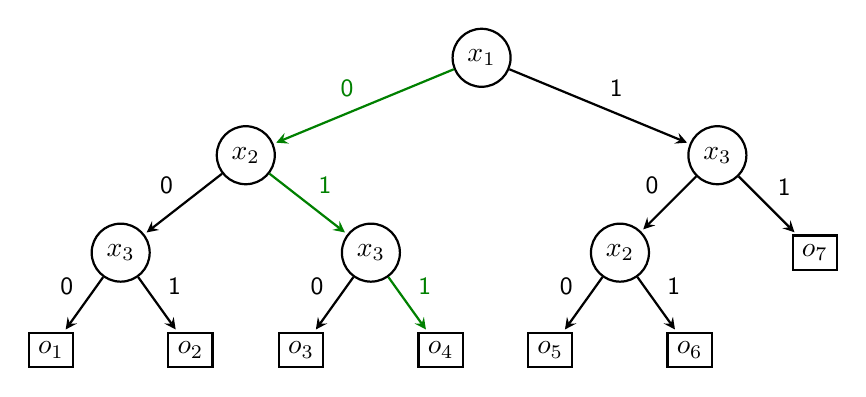
\begin{tikzpicture}[->,>=stealth,shorten >=1pt,auto,node distance=1.75cm, thick,main node/.style={scale=0.9,circle,draw,font=\sffamily\normalsize}]

        \node[circle, draw] (1)[] {$x_1$};

        \node[circle, draw] (2) [below left of=1, xshift=-50, ]{$x_2$};
        \node[circle, draw] (3) [below right of=1, xshift=50, ]{$x_3$};

        \node[circle, draw] (4) [below left of=2, xshift=-10, ]{$x_3$};
        \node[circle, draw] (5) [below right of=2, xshift=10, ]{$x_3$};
        \node[circle, draw] (6) [below left of=3, ]{$x_2$};
        \node[rectangle, draw] (7) [below right of=3]{$o_7$};

        \node[rectangle, draw] (8) [below left of=4, xshift=10]{$o_1$};
        \node[rectangle, draw] (9) [below right of=4, xshift=-10]{$o_2$};
        \node[rectangle, draw] (10) [below left of=5, xshift=10]{$o_3$};
        \node[rectangle, draw] (11) [below right of=5, xshift=-10]{$o_4$};
        \node[rectangle, draw] (12) [below left of=6, xshift=10]{$o_5$};
        \node[rectangle, draw] (13) [below right of=6, xshift=-10]{$o_6$};

        \path[every node/.style={font=\sffamily\small}]
        (1) edge[swap, color=Green]  node{0} (2)
        (1) edge node{1}(3)

        (2) edge[swap]  node{0} (4)
        (2) edge[color=Green]  node{1}(5)

        (3) edge[swap]  node{0} (6)
        (3) edge  node{1}(7)
                    
        (4) edge[swap]  node{0} (8)
        (4) edge  node{1}(9)

        (5) edge[swap]  node{0} (10)
        (5) edge[color=Green]  node{1}(11)

        (6) edge[swap]  node{0} (12)
        (6) edge  node{1}(13)
        ;
    \end{tikzpicture}

    \caption{An example of a decision tree of size 13 and depth 3. The green path shows the computation made for the input $x = 011$.}
    \label{fig:decision_tree}
\end{figure}

\cleardoublepage
\chapter{Proof complexity} \label{chap:proof_complexity}

\section{Propositional proof systems}

Proof complexity is the branch of computational complexity and logic that studies the resources that are needed in order to \emph{certify} mathematical statements, rather than of the resources needed to \emph{decide} them. At its core, proof complexity asks if there is a way of writing down proofs of propositional tautologies so that every tautology has short proofs. Such ways of proof writing can be viewed as sets of rules capable of manipulating propositional formulas, deriving new formulas from them. These sets of rules are referred to as \textit{propositional proof systems}. When a formula $\psi$ can be derived from a formula $\varphi$ through the rules of a proof system $Q$, we write $\varphi \stackrel{Q}{\vdash} \psi$ or simply $\varphi \vdash \psi$ when the context is clear. The easiest example of propositional proof system is \textit{Resolution}, based on two single rules:
\[\dfrac{C \lor x \quad D \lor \lnot{x}}{C \lor D} \quad \text{(resolution)} \qquad\qquad \dfrac{C}{C \lor B} \quad \text{(weakening)}\]

For a more detailed discussion on examples of proof systems, see the next section \todo{add ref}. In the seminal paper from which proof complexity originated, defined proof systems as surjective functions $Q : \Sigma^* \to \mathrm{TAUT}$, where the latter is the set of all tautologies, $\mathrm{TAUT} = \{\abk{\varphi} \mid \varphi \text{ a CNF tautology}\}$. The idea behind this definition is that of an algorithm that is able to determine which tautology is proven by a given proof. A modern and more descriptive definition can be achieved through the concept of verifier.

\begin{definition}
    A propositional proof system (p.p.s.) is a verifier $Q$ such that for all formulas $\varphi$ it holds that $\varphi \in \mathrm{TAUT}$ if and only if there is a proof $\pi \in \Sigma^*$ such that $Q(\varphi, \pi) = 1$ and $Q$ runs in time $O((\abs{\varphi} + \abs{\pi})^c)$ for some $c > 0$.
\end{definition}

This if and only if definition can be split in two implications called completeness and soundness. A proof system $Q$ is \textit{complete} if whenever a formula has a $Q$-proof it also is a tautology. Vice versa, $Q$ is \textit{sound} if whenever a formula is a tautology it also has a $Q$-proof. When $\pi$ is a $Q$-proof of $\varphi$, we often write $\pi : Q \vdash \varphi$.

When for each tautology there is a short proof, i.e. $\abs{\pi} = O(\abs{\varphi}^c)$ for some $c > 0$, we say that the proof system is \textit{polynomially bounded}. Proof systems were originally introduced by Cook and Reckhow as a possible way of attacking the $\mathsf{NP}$ vs. $\mathsf{coNP}$ problem. In fact, through the modern definition, its immediate to see that finding a polynomially bounded p.p.s. is equivalent to proving that $\mathsf{NP} = \mathsf{coNP}$.

\begin{proposition}
    There is a polynomially bounded p.p.s. if and only if $\mathsf{NP} = \mathsf{coNP}$ 
\end{proposition}

\begin{proof}

    One can easily prove that $\mathrm{TAUT}$ is $\mathsf{coNP}$-complete. For our purposes, we can omit this proof and assume it to hold. Let $Q$ be a polynomially bounded p.p.s. Then, since for each formula there is a proof of size $\abs{\pi} = O(\abs{\varphi}^c)$ for some $c > 0$, $Q$ is a verifier for $\mathrm{TAUT}$ with polynomial runtime with respect to the input size $\abs{\varphi}$, concluding that $\mathrm{TAUT} \in \mathsf{NP}$. By completeness, we get that $\mathsf{NP} = \mathsf{coNP}$.

    Vice versa, suppose that $\mathsf{NP} = \mathsf{coNP}$. Then, since $\mathrm{TAUT} \in \mathsf{NP}$, there is a polynomial time verifier $V$ for $\mathrm{TAUT}$. In order for it to run in polynomial time, for each formula $\varphi$ there must be at least one witness $t$ such that $\abs{w} = O(\abs{\varphi}^d)$ for some $d > 0$, otherwise reading the witness would always require super-polynomial runtime, raising a contradiction. This concludes that $V$ is a polynomially bounded p.p.s.
\end{proof}

In their programme, Cook and Reckhow outlined a possible roadmap to proving that $\mathsf{NP} \neq \mathsf{coNP}$ through p.p.s. Their idea involved proving that strong proof systems require super-polynomial size proofs for some formulas, to then generalize the various results to any possible proof system, i.e. showing that every proof system has at least one formula that is hard to prove. However, researchers quickly realized that this task would be tedious even for weaker systems. In fact, even after almost 40 years of research in the field, only a few weak systems have been completely outlined (e.g. Resolution). 

The programme has also a second, entirely practical, motivation. Every complete
algorithm that established the satisfiability of a propositional formul, referred to as a \textit{SAT-solver}, implicitly produces a proof of that formula in some proof system. For instance, the DPLL algorithm (Davis-Putnam-Logemann-Loveland) and CDCL solvers (Conflict-driven Clause Learning) produce resolution proofs, while Gr\"obner basis
solvers produce algebraic proofs. A lower bound on proof size in a system
is therefore an unconditional lower bound on the running time of \emph{every}
algorithm of the corresponding kind, regardless of how cleverly it is
implemented. Proof complexity is, from this point of view, the theory of the
limits of automated reasoning.

\section{Common proof systems}

\subsection{Resolution}

The Resolution proof system ($\mathrm{Res}$), introduced by Robinson \todo{add ref}, is the most extensively studied proof system, extensively in automated theorem proving, SAT-solvers and artificial intelligence. Like many weak proof systems, Resolution's proofs are actually \textit{refutations}, i.e. \curlyquotes{proofs} of unsatisfiability of a formula. This is a feature, not an issue: since $\varphi$ is a tautology if and only if $\lnot \varphi$ is unsatisfiable, any refutation of $\lnot \varphi$ is actually a proof of $\varphi$. In many works, the word refutation is often used as a synonym of proof. To help the reader, this won't be the case in this work.

Resolution refutations are based on repeated applications of two simple rules, starting from the axioms of the initial formula:
\[\dfrac{C \lor x \quad D \lor \lnot{x}}{C \lor D} \quad \text{(resolution)} \qquad\qquad \dfrac{C}{C \lor B} \quad \text{(weakening)}\]

Given a CNF formula $\varphi = C_1 \land \ldots \land C_m$, let $\mathrm{Ax}(\varphi) = \{C_1, \ldots, C_m\}$ be the set of axioms of $\varphi$. Then, a Resolution refutation of $\varphi$ is a sequence of clauses $\pi = (D_1, D_2, \ldots, D_t)$ such that for each $i \in [t]$ exactly one of the following holds:
\begin{itemize}
    \item \textit{Axiom}: $D_i \in \mathrm{Ax}(\varphi)$;
    \item \textit{Resolution}: $D_i = \mathrm{Res}(D_j, D_k)$ with $j,k \in [i-1]$;
    \item \textit{Weakening}: $D_i = \mathrm{Weak}(D_j)$ with $j \in [i-1]$.
\end{itemize}

For the last clause $D_t$, it must hold that $D_t = \bot$, where $\bot$ represents the \textit{empty clause}, i.e. the clause that doesn't contain any literal.

\begin{figure}
    \[\begin{array}{rcl}
        D_1 :& \lnot{x_3} & \text{Axiom} \\
        D_2 :& \lnot{x_1} \lor \lnot{x_2} \lor x_3 & \text{Axiom} \\
        D_3 :& x_1 \lor \lnot{x_2} \lor x_3 & \text{Axiom} \\
        D_4 :& \lnot{x_1} \lor \lnot{x_2} & \mathrm{Res}(D_1, D_2) \\
        D_5 :& x_1 \lor \lnot{x_2} & \mathrm{Res}(D_1, D_3) \\
        D_6 :& x_2 \lor x_3 & \text{Axiom} \\
        D_7 :& x_2 \lor \lnot{x_3} & \text{Axiom} \\
        D_8 :& x_2 & \mathrm{Res}(D_6,D_7) \\
        D_9 :& \lnot{x_1} & \mathrm{Res}(D_4, D_8) \\
        D_{10} :& x_1 & \mathrm{Res}(D_5, D_8) \\
        D_{11} :& \bot & \mathrm{Res}(D_9, D_10) \\
    \end{array}\]
    \caption{Example of a Resolution refutation for the formula $(x_2 \lor x_3) \land (x_2 \lor \lnot{x_3}) \land (x_1 \lor \lnot{x_2} \lor x_3) \land (\lnot{x_1} \lor \lnot{x_2} \lor x_3) \land \lnot{x_3}$}
    \label{fig:res_example_1}
\end{figure}

The idea behind the Resolution proof system comes from the propagation of satisfiability underlying the resolution rule and the weakening rule.

\begin{proposition}
    Let $\alpha$ be an assignment. If $\alpha(C \lor x) = 1$ and $\alpha(D \lor \lnot x) = 1$ then $\alpha(C \lor D) = 1$. Similarly, if $\alpha(C) = 1$ then $\alpha(C \lor B) = 1$
\end{proposition}

One can easily prove by induction that if a clause $Z$ is derived through repeated applications of resolution and weakening starting from the axioms then $\alpha(\varphi) = 1$ implies $\alpha(Z) = 1$. When $Z = \bot$, we reach a contradiction since, by definition, the empty clause is unsatisfiable. Therefore, if we're able to derive $\bot$ starting from $\mathrm{Ax}(\varphi)$, we obtain a valid proof of the fact that $\varphi$ must be unsatisfiable. This proves the soundness of Resolution and completeness can be proven in a similar way.

For any fixed natural number $k \in \N$, we define an extension of the Resolution proof system called \textit{Resolution over $k$-DNFs}, denoted $\mathrm{Res}(k)$, first introduced by \todo{add ref}. This proof system works over sets of $k$-DNF formulas, expressed as a disjunction of conjunctions of at most $k$ literals. Its rules are inspired by to those of Resolution, adapting them to manage $k$-DNFs:
\[\begin{array}{rl}
\dfrac{\mathcal{D}_1 \lor \rbk{\bigvee_{j \in J} \ell_j} \quad \mathcal{D}_2 \lor \rbk{\bigwedge_{j \in J} \lnot \ell_j}}{\mathcal{D}_1 \lor \mathcal{D}_2} & \quad \text{(cut)} \\\\

\dfrac{\mathcal{D}_1 \lor \rbk{\bigwedge_{j \in J} \ell_j} \quad \mathcal{D}_2 \lor \rbk{\bigwedge_{j' \in J'} \ell_{j'}}}{\mathcal{D}_1 \lor \mathcal{D}_2 \lor \rbk{\bigvee_{j \in J \cup J'} \ell_j}} &\quad \text{($\land$ introduction)} \\\\

\dfrac{\mathcal{D}_1}{\mathcal{D}_1 \lor \rbk{\bigwedge_{j \in J} \ell_j}} \qquad \dfrac{\mathcal{D} \lor \rbk{\bigwedge_{j \in J \cup J'} \ell_{j}}}{\mathcal{D}_1 \lor \rbk{\bigvee_{j \in J} \ell_j}} &\quad \text{(weakenings)}
\end{array}\]
where $\mathcal{D}_1$ and $\mathcal{D}_2$ are $k$-DNF formulas.

\subsection{Frege systems}

\textit{Frege systems} are a more classical type of propositional proof system, whose proofs are intended to infer tautologies. These proof systems are well known in the classical Logic literature and, furthermore, they work not only with CNF formulas, but also with general Boolean formulas.

Formally, a Frege system is a propositional proof system built from a finite set of axiom schemes and a finite set of rules of inference that can be applied to sets of formulas. An \textit{axiom scheme} is a meta-formula with variables over formulas that can be substituted by any formula. For instance, both $x_1 \land x_2 \to x-1$ and $(x_1 \lor x_2) \land x_2 \to (x_1 \lor x_2)$ are formulas that can be obtained from the axiom schema $(P \land Q) \to Q$, where $P$ and $Q$ are variables over $\mathrm{Fml}(\mathcal{P})$. A \textit{rule scheme} is a typical rule of logical derivation. A prominent example of a schema rule is the \textit{Modus Ponens} (MP), defined as:
\[\dfrac{P \qquad P \to Q}{Q}\]

Modus Ponens allows to cut implications from formulas of the form $P \to Q$ once the formula $P$ alone is derived. We can define different Frege systems introducing different axiom schemes. Nonetheless, Reckhow proved that all Frege systems are polynomially equivalent to each other \todo{add ref}, meaning that the axiom scheme and rule scheme chosen is not relevant, up to some polynomial factor (see Section \todo{add ref} for an explanation of polynomial equivalence). Therefore, we don't actually care about which rules and axioms are used in our Frege system. This allows us to restrict our interest to a standardized Frege system, known in the literature as \textit{Hilbert's propositional proof system}, denoted with $\mathrm{F}$ or $\mathrm{Frege}$. The rule scheme of this proof system allows only the use of Modus Ponens over the following standard axiom scheme $\mathrm{Ax}(\mathrm{F})$ of Hilbert-style systems for propositional logic:

\[\begin{array}{rll}
    (1) \quad & A \to B \to (A \land B) \\
    (2) \quad & (A \land B) \to A & \land \text{ rules} \\
    (3) \quad & (A \land B) \to B \\[1em]
    (4) \quad & A \to (A \lor B) \\
    (5) \quad & B \to (A \lor B) & \lor \text{ rules} \\
    (6) \quad & (A \to C) \to (B \to C) \to ((A \lor B) \to C) \\[1em]
    (7) \quad & (\bot \to A) \\
    (8) \quad & (A \to \bot) \to \neg A & \neg \text{ rules} \\
    (9) \quad & A \to (\neg A \to \bot) \\
    (10) \quad & (\neg A \to \bot) \to A \\[1em]
    (11) \quad & A \to A \\
    (12) \quad & A \to (B \to A) & \to \text{ rules} \\
    (13) \quad & (A \to (B \to C)) \to ((A \to B) \to (A \to C))
\end{array}\]

Given a formula $A$, an F-proof of $A$ is sequence of formulas $\pi = (A_1, \ldots , A_t)$ such that each $i \in [t]$ exactly one of the following holds:
\begin{itemize}
    \item \textit{Axiom}: $A_i \in \mathrm{Ax}(\mathrm{F})$;
    \item \textit{Modus Ponens}: $A_i = \mathrm{MP}(A_j, A_k)$ with $j,k \in [i-1]$.
\end{itemize}

For the last formula $A_t$, it must hold that $A = A_t$. The soundness of F comes immediately from the soundness of Modus Ponens, something that assumed as an axiom in standard settings of classical Logic. Completeness follows similarly.

\textit{Extended Frege systems}, denoted with $\mathrm{EF}$, are Frege systems augmented with an \textit{extension rule} that allows the introduction of new variables that abbreviate more complex formulas.
\begin{itemize}
    \item \textit{Extension}: $A_i = q \leftrightarrow B$ where $q$ is a new variable that never appeared before and $B$ is any propositional formula.
\end{itemize}

Intuitively, this rule allows us to write shorter proofs by encoding partial statements are single variables and use it in the proof, instead of carrying over the initial statement across the whole proof. In some sense, Frege proofs can be viewed as proofs that reason about polynomial size Boolean
formulas, while Extended Frege proofs as proofs that reason about polynomial size Boolean circuits.

\subsection{Algebraic systems}

\textit{Algebraic proof systems} are proof systems based on polynomials. 
These systems can be used to witness the fact that a system of polynomial equations over a the polynomial ring $\F[x_1, \ldots, x_n]$ is unsolvable; equivalently, that the polynomials do not have a common root.

Consider a CNF formula $\varphi$ defined over $x_1, \ldots, x_n$. The formula can be easily encoded as a set of polynomials such that the formulas is unsatisfiable if and only if such set of polynomials has no solution. We map each clause of $\varphi$ to an equation in the following way:
\[\bigvee_{i \in I} x_i \lor \bigvee_{j \in J} \lnot x_j \mapsto \prod_{i \in I} x_i \prod_{j \in J} (1-x_j) = 0\] 

where $I$ and $J$ are, respectively, the set of positive and negative literals of the clause. For each clause $C$, its corresponding polynomial is denoted with $P(C)$. The formula $\varphi$ is unsatisfiable if and only if the system $\Phi = \{P(C)\}_{C \in \varphi} \cup \{x_i^2 - x_i = 0\}_{i \in [n]}$ has no solutions. In particular, the latter set of equations is used to restrict all possible solutions to those that give Boolean values to $x_1, \ldots, x_n$.

After this transformation is made, the question of whether a formula is unsatisfiable is reduced to the question of a set of polynomial equations is unsolvable. Algebraic tools can then be used in order to decide unsatisfiability of the original formulas. We notice that, under this framework, truth is inversely represented: the value $0$ represents truth, while $1$ represents falsity.

Two particular algebraic proof systems are extensively studied in proof complexity: Nullstellensatz and Polynomial Calculus. \textit{Nullstellensatz} (NS) is a static algebraic proof system, i.e. one that doesn't use rules of inference, based on Hilbert's Nullstellensatz, which states that given $m$ polynomials $p_1, \ldots, p_m$ the system $p_1(x) = p_2(x) = \ldots = p_m(x) = 0$ is unsolvable if and only if 1 lies in their generated ideal, i.e. there are $m$ polynomials $g_1, \ldots , g_m$ such that $\sum_{j = 1}^m g_jp_j = 1$. For any CNF $\varphi$, an NS-proof of $\varphi$ is the set of polynomials $\pi = \{g_1, \ldots, g_m, h_1, \ldots, h_m\}$ such that:
\[\sum_{j = 1}^m g_jp_j + \sum_{i = 1}^n h_i(x_i^2-x_i) = 1\]
where $p_j = P(C_j)$ for each $j \in [m]$.

\textit{Polynomial Calculus} (PC) is a dynamic proof system based on two rules:
\[\dfrac{p \qquad q}{\alpha p+ \beta q} \quad \text{(linear combination)} \qquad\qquad \dfrac{p}{xp} \quad \text{(multiplication)}\]
where $\alpha,\beta \in \F$ and $x \in \{x_1, \ldots, x_n\}$. A PC-proof of the CNF $\varphi$ is a sequence of polynomials $\pi = (f_1, \ldots, f_t)$ such that each $i \in [t-1]$ exactly one of the following holds:
\begin{itemize}
    \item \textit{Axiom}: $f_i$ is the polynomial of some equation in $\Phi$
    \item \textit{Linear combination}: $f_i = \mathrm{Sum}(f_j, f_k)$ with $j,k \in [i-1]$
    \item \textit{Multiplication}: $f_i = \mathrm{Mul}(f_j)$ with $j \in [i-1]$
\end{itemize}

For the last polynomial $f_t$, it must hold that $f_t = 1$. The soundness of PC can be proven in way similar to Resolution: if we assume that the system of equations $\Pi$ has a solution, the equality with 0 can be propagated down to the last polynomial $f_t = 1$, raising a contradiction. Completeness follows similarly.

\subsection{Optimization-based systems}

\textit{Optimization-based proof systems} are proof systems based on linear programming. All such proof systems are variants of the \textit{Cutting Planes} (CP) proof system, a refutational method derived from 0-1 integer programming. In CP, any CNF formula $\varphi$ is converted into an equivalent system of linear inequalities (similar to how algebraic systems convert them into equations) whose integer binary solutions correspond directly to the satisfying assignments of $\varphi$. Each clause of a formula $\varphi$ is mapped to an inequality in the following way:
\[\bigvee_{i \in I} x_i \lor \bigvee_{j \in J} \lnot x_j \mapsto \sum_{i \in I} x_i + \sum_{j \in J} (1-x_j) \geq 1\] 

For each clause $C$, its corresponding inequality is denoted with $E(C)$. Interpreting truthness as 1 and falseness as 0, the formula $\varphi$ is unsatisfiable if and only if the system $\Phi  = \{E(C)\}_{C \in \varphi} \cup \{x_i \geq 0; x_i \leq 1\}_{i \in [n]}$ has no an integer solution. The set of all feasible solutions for this system yield a polytope $P$. While any Boolean point in $P$ yields a satisfying assignment for $F$, an unsatisfiable formula $F$ may still leave non-integer (fractional) points within $P$. CP eliminates these fractional solutions using the \textit{Chvátal-Gomory cut rule}. In particular, CP is based on the two following rules:
\[\dfrac{\sum_{i \in [n]} \alpha_i x_i \geq \gamma \qquad \sum_{i \in [n]} \beta_{i} x_{i} \geq \delta}{\sum_{i \in [n]} (\alpha_i + \beta_i) x_i \geq \gamma + \delta} \quad \text{(linear combination)}\]
\[\dfrac{\sum_{i \in [n]}  \eta\alpha_i x_i \geq \gamma}{\sum_{i \in [n]} \alpha_ix_i \geq \floor{\frac{\gamma}{\eta}}} \quad \text{(cut)}\]

Formally, a CP-proof of the CNF $\varphi$ is a sequence of inequalities $\pi = (f_1, \ldots, f_t)$ such that each $i \in [t-1]$ exactly one of the following holds:
\begin{itemize}
    \item \textit{Axiom}: $f_i \in \Phi$
    \item \textit{Linear combination}: $f_i = \mathrm{Sum}(f_j, f_k)$ with $j,k \in [i-1]$
    \item \textit{Multiplication}: $f_i = \mathrm{Cut}(f_j)$ with $j \in [i-1]$
\end{itemize}

For the last inequality $f_t$, it must hold that $f_t : 0 \geq 1$ to ensure a contradiction.

\subsection{Tree-like systems}

Consider again the refutation in \Cref{fig:res_example_1}. To make things easier to read, we can represent this refutation as a Directed Acyclic Graph (DAG) by connecting clauses with lines. These refutations are called \textit{DAG-like refutations}.

\begin{figure}[H]
    \centering
    \resizebox{0.8\hsize}{!}{
        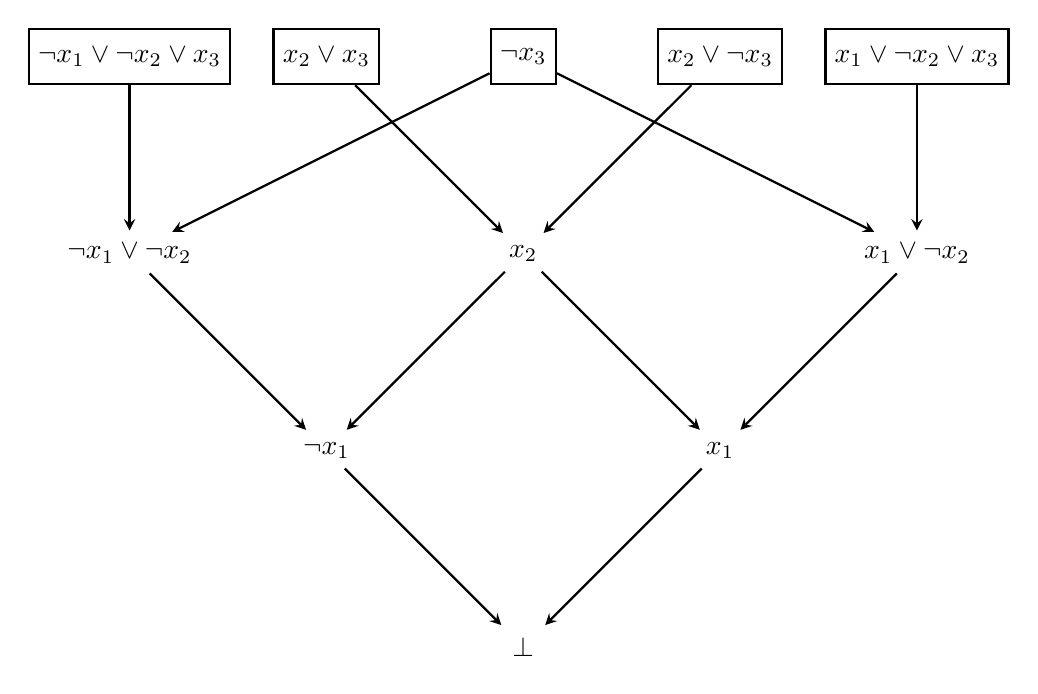
\begin{tikzpicture}[->,>=stealth,shorten >=1pt,auto,node distance=2.5cm, thick,main node/.style={scale=0.9,circle,draw,font=\sffamily\normalsize}]
            \node [rectangle, draw, minimum height=20](1) []{$\lnot{x_1} \lor \lnot{x_2} \lor x_3$};
            \node [rectangle, draw, minimum height=20](2) [right of=1]{$x_2 \lor x_3$};
            \node [rectangle, draw, minimum height=20](3) [right of=2]{$\lnot{x_3}$};
            \node [rectangle, draw, minimum height=20](4) [right of=3]{$x_2 \lor \lnot{x_3}$};
            \node [rectangle, draw, minimum height=20](5) [right of=4]{$x_1 \lor \lnot{x_2} \lor x_3$};

            \node (6) [below of=1]{$\lnot{x_1} \lor \lnot{x_2}$};
            \node (x) [below of=2]{};
            \node (7) [below of=3]{$x_2$};
            \node (y) [below of=4]{};
            \node (8) [below of=5]{$x_1 \lor \lnot{x_2}$};

            \node (9) [below of=x]{$\lnot{x_1}$};
            \node (10) [below of=y]{$x_1$};
            \node (z) [below of=7]{};
            
            \node (11) [below of=z]{$\bot$};
        
            \path[every node/.style={font=\sffamily\small}]
                (1) edge (6)
                (2) edge (7)
                (3) edge (6)
                (3) edge (8)
                (4) edge (7)
                (5) edge (8)

                (6) edge (9)
                (7) edge (9)
                (7) edge (10)
                (8) edge (10)

                (9) edge (11)
                (10) edge (11)
                ;
        \end{tikzpicture}
    }
    \caption{DAG-like representation of the refutation in \Cref{fig:res_example_1}.}
    \label{fig:dag_res_proof}
\end{figure}

We observe that the definition of Resolution refutation allows rules to be applied more than once onto each clause of the proof. There may also be multiple copies of a single clause, each obtained by applying different rules.
When each copy of a clause is used only once as premise in the whole proof, we say that the refutation is \textit{tree-like} (named after the fact that the graph becomes a tree). This restriction implies that if we want to use a clause multiple times then it must be derived again, usually starting from the same axioms.

\begin{figure}[H]
    \centering
    
    \resizebox{1\hsize}{!}{
        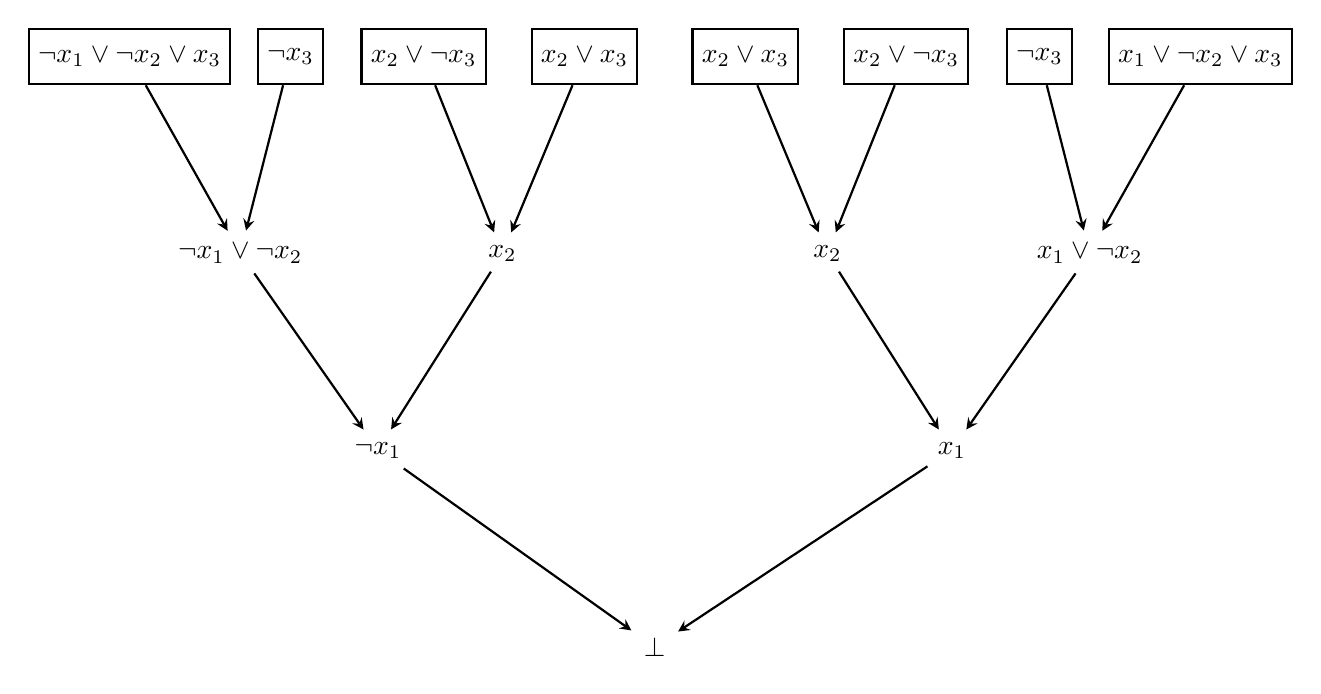
\begin{tikzpicture}[->,>=stealth,shorten >=1pt,auto,node distance=2.5cm, thick,main node/.style={scale=0.9,circle,draw,font=\sffamily\normalsize}]
            \node [rectangle, draw, minimum height=20](1) []{$\lnot{x_1} \lor \lnot{x_2} \lor x_3$};
            \node [rectangle, draw, minimum height=20](2) [right of=1, xshift=-13]{$\lnot{x_3}$};
            \node [rectangle, draw, minimum height=20](3) [right of=2, xshift=-23]{$x_2 \lor \lnot{x_3}$};
            \node [rectangle, draw, minimum height=20](4) [right of=3, xshift=-13]{$x_2 \lor x_3$};
            \node [rectangle, draw, minimum height=20](5) [right of=4, xshift=-13]{$x_2 \lor x_3$};
            \node [rectangle, draw, minimum height=20](6) [right of=5, xshift=-13]{$x_2 \lor \lnot{x_3}$};
            \node [rectangle, draw, minimum height=20](7) [right of=6, xshift=-23]{$\lnot{x_3}$};
            \node [rectangle, draw, minimum height=20](8) [right of=7, xshift=-13]{$x_1 \lor \lnot{x_2} \lor x_3$}; 

            \node (9)[below of=1, xshift=40]{$\lnot{x_1} \lor \lnot{x_2}$};
            \node (10)[below of=3, xshift=28.5]{$x_2$};
            \node (11)[below of=6, xshift=-28.5]{$x_2$};
            \node (12)[below of=8, xshift=-40]{$x_1 \lor \lnot{x_2}$};

            \node (13)[below of=10, xshift=-45]{$\lnot{x_1}$};
            \node (14)[below of=11, xshift=45]{$x_1$};

            \node (15)[below of=13, xshift=100]{$\bot$};
        
            \path[every node/.style={font=\sffamily\small}]
                (1) edge (9)
                (2) edge (9)
                (3) edge (10)
                (4) edge (10)
                (5) edge (11)
                (6) edge (11)
                (7) edge (12)
                (8) edge (12)

                (9) edge (13)
                (10) edge (13)
                (11) edge (14)
                (12) edge (14)

                (13) edge (15)
                (14) edge (15)
                ;
        \end{tikzpicture}
    }
    
    \caption{Tree-like adaptation of the refutation in \Cref{fig:res_example_1}.}
    \label{fig:treelike_res_proof}
\end{figure}

This sub-system of Resolution is called \textit{tree-like Resolution}, denoted with $\mathrm{Res}^*$. The same idea can also be applied to other dynamic systems, obtaining sub-systems like $\mathrm{Res}^*(k), \mathrm{F}^*$ and $\mathrm{PC}^*$. Generally, tree-like sub-system require longer proofs due to the impossibility of reusing derived clauses.

\section{Simulations between proof systems}

To compare the relative strength of different propositional proof systems, we introduce the notion of efficient simulation. This notion comes in a natural way by adapting the idea of polynomial time reduction.

\begin{definition}
    Given two proof systems $P,Q$, we say that $Q$ polynomially simulates $P$, written $P \leq_p Q$ if there is a polynomial time computable function $f : \Sigma^* \to \Sigma^*$ such that for all tautologies $\varphi$ if $\pi$ is a $P$-proof of $\varphi$ then $f(\pi)$ is a $Q$-proof of $\varphi$.
\end{definition}

Intuitively, this means that there is an efficient algorithms transforming $P$-proofs into $Q$-proofs for the same formula. Consider the binary relation $\leq_p$. Similarly to reductions, this formula forms a partial order. In particular, for any pair $P,Q$ of proof systems we say that:
\begin{itemize}
    \item $P$ and $Q$ are \textit{polynomially equivalent} when $P \leq_p Q$ and $Q \leq_p P$. We often write $P \equiv_p Q$ when this holds.
    \item $P$ is \textit{superpolynomially weaker} than $Q$ when $P \leq_p Q$ but $Q \not\leq_p P$
    \item $P$ and $Q$ are \textit{incomparable} when $P \not\leq_p Q$ and $Q \not\leq_p P$
\end{itemize}

It's easy to see that for any dynamic proof system $Q$ it holds that $Q^* \leq_p Q$ since any $Q^*$-proof is also a $Q$-proof. Vice versa, however, it commonly holds that $Q \not\leq_p Q^*$, making tree-like systems typically weaker than their DAG-like counterpart. For instance, standard techniques can prove that the Ordering Principle formula $\mathrm{OP}_n$ is an hard formula for tree-like Resolution but an easy one for Resolution, implying that $\mathrm{Res} \not\leq_p \mathrm{Res}^*$.

When it comes to comparing Resolution with Nullstellensatz and Polynomial Calculus, they're both incomparable with it. This is due to the fact that negative literals easily blow up the size of the proof due to the increase in the number of monomials when expanded. To fix this, we can consider a variant of Polynomial Calculus referred to as \textit{Polynomial Calculus with Resolution} (PCR) -- a name that pretty much says it all -- where for each variable $x_i$ we add a new variable $\overline{x_i}$ in order to map negative literals $\lnot x_i$ directly to this new variable.
\[\bigvee_{i \in I} x_i \lor \bigvee_{j \in J} \lnot x_j \mapsto \prod_{i \in I} x_i \prod_{j \in J} \overline{x_j} = 0\]

All the other standard simulations and separations between proof systems are omitted and summarized in \Cref{fig:simulations}.

\begin{figure}[H]
    \centering
    \resizebox{0.5\textwidth}{!}{
        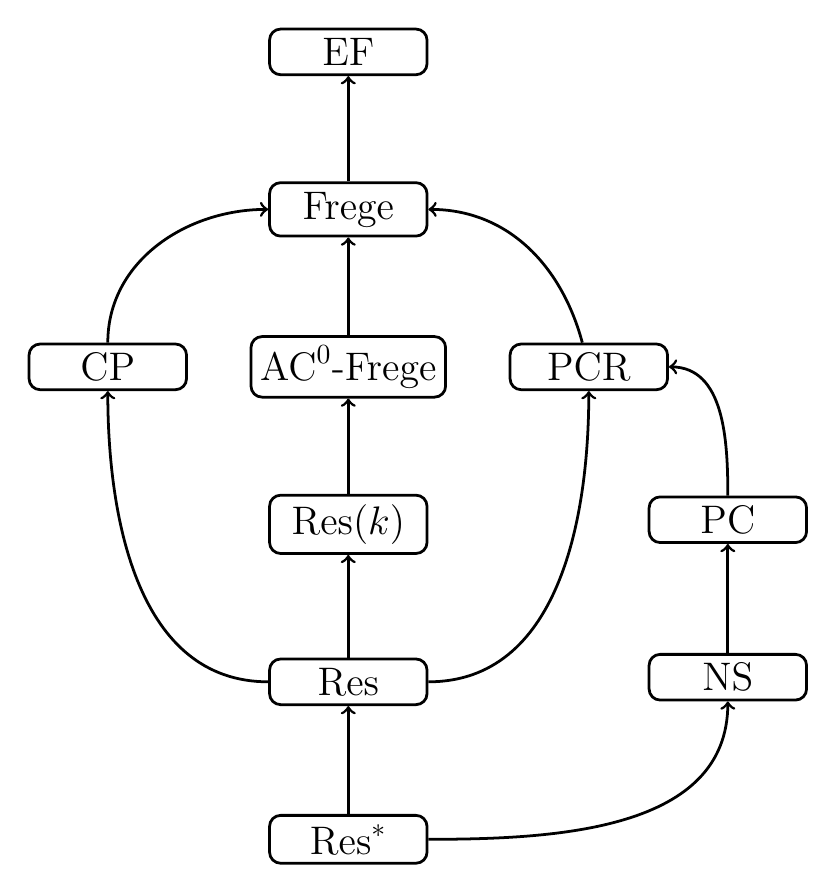
\begin{tikzpicture}[node distance=2cm and 1.8cm, font=\Large, line width=1pt ]
            % --- Nodes Placement ---
            \node[rectangle, rounded corners, draw, minimum width = 2cm] (EF) {$\mathrm{EF}$};
            \node[rectangle, rounded corners, draw, minimum width = 2cm] (F) [below of = EF] {$\mathrm{Frege}$};
            \node[rectangle, rounded corners, draw, minimum width = 2cm] (AC0F) [below of = F] {$\mathrm{AC}^0$-$\mathrm{Frege}$};
            \node[rectangle, rounded corners, draw, minimum width = 2cm] (ResK) [below of = AC0F] {$\mathrm{Res}(k)$};
            \node[rectangle, rounded corners, draw, minimum width = 2cm] (Res) [below of = ResK] {$\mathrm{Res}$};
            
            \node[rectangle, rounded corners, draw, minimum width = 2cm] (CP) [left of = AC0F, xshift = -30] {$\mathrm{CP}$};
            \node[rectangle, rounded corners, draw, minimum width = 2cm] (PCR) [right of = AC0F, xshift = 30] {$\mathrm{PCR}$};
            \node[rectangle, rounded corners, draw, minimum width = 2cm] (PC) [below right of = PCR, xshift=10, yshift=-15] {$\mathrm{PC}$};
            \node[rectangle, rounded corners, draw, minimum width = 2cm] (NS) [below of = PC] {$\mathrm{NS}$};
            \node[rectangle, rounded corners, draw, minimum width = 2cm] (ResStar) [below of = Res] {$\mathrm{Res}^*$};

            % --- Direct Straight Connections ---
            \draw[->] (Res) -- (ResK);
            \draw[->] (ResK) -- (AC0F);
            \draw[->] (AC0F) -- (F);
            \draw[->] (F) -- (EF);
            
            \draw[->] (ResStar) -- (Res);
            \draw[->] (NS) -- (PC);
            
            % --- Curved Connections ---
            \draw[->] (ResStar) to[out=0, in=270] (NS);
            \draw[->] (Res) to[out=180, in=270] (CP);
            \draw[->] (Res) to[out=0, in=270] (PCR);

            \draw[->] (PC) to[out=90, in=0] (PCR);
            \draw[->] (CP) to[out=90, in=180] (F);
            \draw[->] (PCR) to[out=105, in=0] (F);
        \end{tikzpicture}
    }
    
    \caption{Simulations between standard proof systems.}
    \label{fig:simulations}
\end{figure}
\todo{add references for simulations (also inside the image)}

\section{Complexity measures for proof systems}

Complexity measures lie at the heart of proof complexity. These measures provide a rigorous language to measure if a minimal proof must be short or long, allowing us to evaluate how different systems perform on proving a common statement. Different measures highlight different facets of a proof, often interlinking them. By analyzing these measures, we gain a deeper understanding of the inherent difficulty of logical reasoning, even from an algorithmic prospective.

Resolution is the quintessential proof system when it comes to complexity measures. Consider a Res-proof $\pi$. For any clause $C$, let $\abs{C}$ denote the number of literals in $C$. Our main complexity measure of interest is The \textit{size} of $\pi$, written as $\abs{\pi}$, corresponding to the total number of literals inside it, i.e. $\abs{\pi} = \sum_{D_i \in \pi} \abs{D_i}$. For instance, the refutation in \Cref{fig:res_example_1} has size $19$. In a natural way, the size of the proof corresponds to the number of symbols used to describe the witness of the verifier-based definition of the proof system. For any formula $\varphi$ with $m$ clauses over $n$ variables, the Resolution size of $\varphi$, written as $\mathrm{size}_{\mathrm{Res}}(\varphi)$, is the minimum size across all Res-proofs of $\varphi$ (equivalently, across all refutations of $\lnot \varphi$).
\[\mathrm{size}_{\mathrm{Res}}(\varphi) = \min_{\pi : \mathrm{Res} \vdash \varphi} \abs{\pi}\]

Finding the Resolution size of a formula tells us the exact minimum number of symbols in a witnessing string for the given formula. Proving the existence of at least one formula $\varphi$, with $m$ clauses over $n$ variables, whose Resolution size is super-polynomial with respect to $\abs{\varphi} = \Theta(n+m)$ is sufficient to conclude Resolution is not polynomially bounded. Haken \todo{add ref} was the first to show that one such formula is the Pigeonhole Principle formula $\mathrm{PHP}^{n+1}_{n}$, which has size $2^{\Theta(n)}$. This result not only implies that Resolution is polynomially bounded, but it also implies that every CNF formula that implicitly describes the Pigeonhole Principle is hard for Resolution. Since this combinatorial principle is at the foundation of mathematics, this makes Resolution weak against a wide subset of formulas. 

A natural complexity measure related with size is the \textit{length} of a proof, which measures the total number of clauses inside $\pi$, i.e. the number of steps in the proof. The Resolution length of a formula $\varphi$, written as $\mathrm{length}_{\mathrm{Res}}(\varphi)$, is the minimum length across all Res-proofs of $\varphi$. One can easily prove that $\mathrm{length}_{\mathrm{Res}}(\varphi) \leq \mathrm{size}_{\mathrm{Res}}(\varphi) \leq n \cdot \mathrm{length}_{\mathrm{Res}}(\varphi)$ holds for any $\varphi$. For this reason, the concepts of size and length are often treated as synonyms in the case of Resolution. 

Another complexity measure inspired by Haken's proof is the \textit{width} of a proof $\pi$, defined as the maximum number of literals across all clauses of $\pi$, i.e. $\max_{D_i \in \pi} \abs{D_i}$. The Resolution width of $\varphi$, written as $\mathrm{width}_{\mathrm{Res}}(\varphi)$, is defined as the minimum across all proofs. Ben-Sasson and Widgerson \todo{add ref} proved that Resolution size and width are related one another through the trade-off.

\begin{theorem}
    $\mathrm{size}_{\mathrm{Res}}(\varphi) = \exp \left (\Omega \left (\frac{(\mathrm{width}_{\mathrm{Res}}(\varphi) - \mathrm{width}(F))^2}{n}\right ) \right )$
\end{theorem}

We observe that in the exponent of the right hand side of the equation we have the difference between the Resolution width and the width of the axioms in $\varphi$. Because of this, for the case of families of formulas with large initial clauses, like the Pigeonhole Principle formula $\mathrm{PHP}^{n+1}_n$, this method can prove only trivial size lower bounds (in fact, Haken's proof uses width of \textit{monotone} clauses).

All Resolution measures carry over to $\mathrm{Res}^*, \mathrm{Res}(k)$ and $\mathrm{CP}$, with some small variations: in $\mathrm{Res}(k)$ the concept of width translates to the number of $k$-DNFs inside the conjunctions, while in $\mathrm{CP}$ there is no real concept of width. These adaptations imply that the above trade-off theorem doesn't have an analogous in these two worlds. 

Moving to other proof systems, size and length measures are inherited by Frege systems in a natural way, but the relation between $\mathrm{size}_{\mathrm{Frege}}(\varphi)$ and $\mathrm{length}_{\mathrm{Frege}}(\varphi)$ and length is not so straightforward anymore since the formulas inside the proof are not restricted to being clauses. Nonetheless, Reckhow \todo{add ref} proved that they are still polynomially related one another.
\begin{theorem}
    $\mathrm{size}_{\mathrm{Frege}}(\varphi) = O(\mathrm{length}_{\mathrm{Frege}}(\varphi) \cdot (\abs{\varphi} + \mathrm{length}_{\mathrm{Frege}}(\varphi))^2)$
\end{theorem}

Other then this, no general trade-offs are known for Frege systems. In addition, there is no concept of width (again, formulas are not restricted to being clauses). Nonetheless, there is another complexity measures of our interest called \textit{nested depth}, that being the maximum nesting level of logical connectives across all formulas of the proof. For general Frege system, there are no known formulas that require exponential size proofs. However, when restricted to $\Theta(1)$ nested depth, some formulas are known. This sub-system of Frege is known as $\mathrm{AC}^0$-Frege. Furthermore, it can be easily proven that Frege is equivalent to Resolution when restricted to depth-1 formulas.

Both in Nullstellensatz and Polynomial Calculus, size is defined differently. The size of a polynomial $\norm{p}$ is defined as the number of non-zero monomials when expanded out as a linear combination of monomials. The size of a proof $\norm{\pi}_Q$, with $Q \in \{\mathrm{NS}, \mathsf{PC}\}$, is the sum of the sizes of all the polynomials inside it. Regarding polynomials, we have another complexity measure: \textit{degree}. The degree of a polynomial $\deg(p)$ is the maximum degree of all monomials inside it. The degree of a proof is $\mathrm{deg}_Q(\pi)$ is the maximum degree across all polynomials inside it. The values of $\mathrm{size}_{Q}(\varphi)$, $\mathrm{deg}_{Q}(\varphi)$ and are defined accordingly. 

In particular, for a NS-proof $\pi = \{g_1, \ldots, g_m, h_1, \ldots, h_n\}$ over the system $\{p_1, \ldots, p_m\} \cup \{x_i^2 - x_i\}_{i \in [n]}$ the size and degree of $\pi$ are defined by:
\[\norm{\pi}_{\mathrm{NS}} = \sum_{j = 1}^m \norm{g_h} \norm{p_j} + \sum_{i = 1}^n 2\norm{h_i}\]
\[\mathrm{deg}_\mathrm{NS}(\pi) = \max_{j \in [m], i \in [n]} (\deg(g_j) + \deg(p_j), 2 + \deg(h_i))\]

For a PC-proof $\pi' = (f_1, \ldots, f_t)$, instead, the size of $\pi'$ is defined as $\norm{\pi'}_{\mathrm{PC}} = \sum_{i = 1}^t \norm{f_i}$ and the degree is $\max_{i \in [t]} (\deg(f_i))$.

\section{Game characterizations of Resolution measures}

\subsection{The Prover-Delayer Game (TODO)}

\subsection{The Spoiler-Duplicator Game (TODO)}

\cleardoublepage

\chapter{Automatability} \label{chap:automatability}

\cleardoublepage

\chapter{Analyzability (TODO)} \label{chap:analyzability}

\section{Do proofs of $\lnot \mathrm{Ref}$ leak information?}

\section{Analyzability of Resolution}

\subsection{Reducing block-width in $\mathrm{Ref}$ proofs}

\subsection{Extracting assignments from narrow $\mathrm{Ref}$ proofs}

\section{Extending analyzability up to PCR}

\section{Analyzability and feasible interpolation}



\cleardoublepage


% % ================== NOTES ==================
% \chapter{Notes} \label{chap:notes}


    \begin{definition}[Proof Analysis Problem]
        Given a proof system $Q$, the Proof Analysis Problem over $Q$ restricted to $s(n)$ is defined as:
        \[\mathrm{PAP}_Q[s(n)] = \{(\varphi, \pi, 1^t) \mid \varphi \in \mathrm{Sat}, \pi : Q \vdash \lnot \mathrm{Ref}^\mathrm{Res}(\varphi, s) \text{ with } t \geq s(n), \abs{\varphi} = n\}\]
    \end{definition}

    \begin{definition}[Proof Size Problem]
        Given a proof system $Q$, the Proof Size Problem over $Q$ is defined as:
        \[\mathrm{PSP}_Q = \{(\varphi, 1^t) \mid \exists \pi \text{ s.t. } \pi : Q \vdash \phi, \abs{\pi} \leq t\}\]
    \end{definition}

    For any proof system $Q$, the automatability of $Q$ can be viewed as some form of search version of $PSP_Q$, where $t$ is forced to be in function of $\abs{\varphi} + \mathrm{Size}_Q(\varphi)$.
    

    \begin{definition}[Automatability]
        A proof system $Q$ is said to be $t$-\textit{automatable} when there is an algorithm $\mathcal{A}$ such that $\mathcal{A}(\varphi)$ returns a $Q$-proof of the formula $\varphi$ in time at most $t(\abs{\varphi} + \mathrm{Size}_Q(\varphi))$.
    \end{definition}

    When $t = \mathrm{poly}$, we simply say that $Q$ is \textit{automatable}.


    \begin{definition}[Analyzability]
        A proof system $Q$ is said to be $(t,s)$-\textit{analyzable} when $\mathrm{PAP}_Q[s(n)] \in \mathsf{DTIME}(t(n))$.
    \end{definition}

    When $t,s = \mathrm{poly}(n)$, we simply say that $Q$ is \textit{analyzable}.


    It's immediate to see that automatability and analyzability can be combined to easily solve the satisfiability problem.

    \begin{proposition}
        Let $Q$ be a proof system such that $\mathrm{Res} \leq Q$. If $Q$ is $t$-automatable and $(t,t)$-analyzable then $\mathsf{NP} \subseteq \mathsf{DTIME}(t(n))$.
    \end{proposition}

    \begin{proof}
        Let $\mathcal{A}$ and $\mathcal{B}$ be two algorithms certifying, respectfully, that $Q$ is $t$-automatable and $(t,t)$-analyzable. Then, the algorithm $\mathcal{C}(\phi) = \mathrm{B}(\phi, \mathcal{A}(\phi), \abs{\phi}^2)$
    \end{proof}

    Under the standard complexity assumption that $\mathrm{NP}$ is not contained in $\mathsf{P}$ (or $\mathsf{QP}$, $\mathsf{SUBEXP}$), the properties of automatability and analyzability are disjoint when restricted to polynomial time algorithms (or quasi-polynomial, sub-exponential). We observe that, even if the above statement holds for proof systems that simulate Resolution, the disjointness of both properties under polynomial time algorithms seems to hold even for proof systems weaker than Resolution. For instance, de Rezende [dR20] proved that, under the Randomized Exponential Time Hypothesis (rETH), tree-like Resolution doesn't admit automating algorithms with runtime lower than quasi-polynomial.

\cleardoublepage

% ================== CONCLUSIONS ==================
\chapter*{Conclusions}

\addcontentsline{toc}{chapter}{Conclusions}

We proved that Polynomial Calculus with Resolution is analyzable, and hence so are Nullstellensatz and Polynomial Calculus, by lifting the block-width argument to block-degree. As a corollary, we obtained a new proof that automating PCR is $\mathsf{NP}$-hard. We then compared analyzability with feasible interpolation. Proving that interpolation implies analyzability would show that Resolution is not weakly automatable unless $\mathsf{P}$ = $\mathsf{NP}$, while for every disjoint $\mathsf{NP}$-pair there is an analyzable system, simulating Resolution and closed under restrictions, that has feasible interpolation only if the pair is polynomial-time separable. Any connection between the two notions must therefore use specific properties of natural proof systems. Several questions that further research may explore remain open.

\textit{Search-analyzability of PCR}. The most immediate question left open is whether a satisfying assignment of $\varphi$ can be extracted in polynomial time from a short PCR proof of $\lnot\mathrm{Ref}_s(\varphi)$.

\textit{Pudlák's upper bound in algebraic systems}. Our proof that automating PCR is $\mathsf{NP}$-hard uses Pudlák's upper bound for Resolution, which PCR inherits because it simulates Resolution. Nullstellensatz and Polynomial Calculus do not simulate Resolution efficiently, so the same argument does not give the $\mathsf{NP}$-hardness of automating them, even though both are analyzable by our result. It is open whether $\mathrm{Ref}_s(\varphi)$, or a suitable algebraic variant of it, has short Polynomial Calculus or Nullstellensatz refutations when $\varphi$ is satisfiable. A positive answer, combined with our analyzability results, would give a direct proof that automating these systems is $\mathsf{NP}$-hard along the lines of Atserias and Müller.

\textit{Analyzability of Cutting Planes, Res(k) and bounded-depth Frege}. Every analyzability result needs a lower bound for $\mathrm{Ref}_s(\varphi)$ in the analyzed system. For Res(k), the block-width technique may extend through switching lemmas for k-DNFs. For Cutting Planes, the usual techniques are lifting from communication complexity and monotone interpolation, and it is unclear whether either adapts to $\mathrm{Ref}_s(\varphi)$. For bounded-depth Frege, switching-lemma lower bounds for the pigeonhole principle exist, but the retraction version would need a separate analysis.

\textit{A natural separation of analyzability and interpolation}. We showed that analyzability and feasible interpolation are different in general, but the separating system is artificial. Is there a natural analyzable proof system without feasible interpolation, or a natural system with feasible interpolation that is not analyzable? Cutting Planes is the natural candidate for the second question, since it has feasible interpolation through monotone real circuits and its analyzability is open. A proof that Cutting Planes is not analyzable under a standard assumption would give the first natural separation. A proof that it is analyzable would extend the known coincidence of the two properties to a system that is incomparable with PCR.

\textit{Does interpolation imply analyzability on restricted systems?} Proposition 5.6 rules out a general proof that feasible interpolation implies analyzability, unless the weak automatability of Resolution is settled. It does not rule out such a proof for restricted classes of systems. A natural candidate is the class of systems that extend Resolution, are closed under restrictions and in which lines are evaluated by a bounded number of Boolean functions, such as Res(k). A result of this kind would explain why every analyzable system known before this thesis also has feasible interpolation.

\textit{Weak automatability of Resolution}. The relationship between analyzability and interpolation is tied to the weak automatability of Resolution, one of the central open problems of the area. Weak automatability asks for an algorithm that finds a proof in some possibly stronger system, so the meta-complexity method does not apply directly: the stronger system may refute $\mathrm{Ref}_s(\varphi)$ efficiently even when $\varphi$ is unsatisfiable. Any progress on analyzability for systems above Resolution, such as Res(2), therefore bears directly on this problem.

% ================== ACKNOWLEDGMENTS ==================
% \chapter*{Acknowledgements}
% \addcontentsline{toc}{chapter}{Acknowledgements (TODO)}


\backmatter
\phantomsection

% ================== BIBLIOGRAPHY ==================

\addcontentsline{toc}{chapter}{Bibliography}  % Add Bibliography to ToC
\printbibliography

\end{document}